\documentclass[10pt]{article}
\usepackage{mmmemo}
\usepackage{array}
\usepackage{float}
\usepackage{listings}
\graphicspath{{../../output/pdf/metablate/}}
\setmmlogo{/Users/jvi019/src/mm_memos/assets/uit-circular-logo.pdf}
\showscriptprovenance % Use \hidescriptprovenance to hide script names.
\captionsetup{font=normalsize}
\lstset{basicstyle=\ttfamily\small,breaklines=true,columns=fullflexible,keepspaces=true}
\mmmemo{VIBE-01}{September 11, 2026}{Juha-Pekka Vierinen}{Vibe implementation and validation record}{Vibe: SiO ablation port and validation}

\begin{document}
\makemmmemo

\mmsection{1. Verdict: a useful scientific program, not yet a complete platform}

Vibe successfully executed a substantially more demanding workload than Hello
World or an FFT: coupled thermal ablation, adaptive integration, event detection,
geodetic transformations, nested threshold searches, and parameter sweeps.
The resulting program consists of \textbf{21 semantic functions} in one
\texttt{metablate.vibepack}. The full run completed \textbf{521 study trajectories},
\textbf{22 cached boundary searches}, and \textbf{260 numerical assertions}.
Search-internal trajectories and validation/refinement runs are additional to
the 521. Eight study figures were produced in both PNG and SVG.

\begin{mmconclusion}
The task demonstrates that the extended Vibe bootstrap can express and execute
a real numerical model accurately and quickly on a CPU. It does not establish
full metablate compatibility, general numerical uncertainty certification,
accelerator portability, large-project scaling, or improved LLM productivity.
Those remain separate acceptance gates.
\end{mmconclusion}

\mmsection{2. What was actually ported}

The implemented scope is the Kero--Szasz thermal-ablation path used by the local
\texttt{ablatemm} SiO studies, rather than every public API in the metablate
package. The original source and saved study products were left unchanged.

\begin{center}
\begin{tabular}{@{}p{1.30in}p{5.53in}@{}}
\toprule
Layer & Implementation and boundary \\
\midrule
Physics & Vibe mass loss, heat balance, drag/scalar gravity, particle mass,
local escape speed, radiation pressure and Poynting--Robertson quantities. \\
Numerics & Vibe Dormand--Prince 5(4), adaptive steps, dense event interpolation,
mass/temperature objectives, bracket expansion and bisection. \\
Geometry / air & Vibe WGS84 conversions, fixed ray and log-density interpolation.
NRLMSIS 2.1 supplies a fixed external input table; MSIS itself is not ported. \\
Host / evidence & Python allocates buffers, calls native entry points, stores
HDF5, plots, and runs an independent original-RHS/SciPy reference. It supplies
no ODE or optimization callbacks to the delivered Vibe studies. \\
Excluded & Alternative metablate models, plasma, sputtering, general dynamic
transfer-coefficient machinery, and the complete Python package interface. \\
\bottomrule
\end{tabular}
\end{center}

\mmsection{3. What Vibe had to learn}

This was not a port onto an unchanged language. The compiler needed boolean
comparisons, scoped \texttt{if}/\texttt{else} and \texttt{while}, typed scalar
math intrinsics, checked numeric casts, and runtime bounds checks for indexed
reads and writes. These were carried through the semantic API, type checker,
query projections, precision traversal, import parser and C backend. The native
build disables floating-point contraction and links platform libm.

The port is authored through a typed Python IR builder and atomic environment
transactions, not through edited \texttt{.vibe} text. Generated C is disposable
compiler output. JSON is transient tool transport, not a forest of persisted
program files. This is a workable agent-facing route, but a bespoke authoring
helper and manual ABI schema still expose missing standard-library/tooling work.

\newpage
\mmsection{4. Physical model and numerical choices}

Let $m$, $v$, $s$ and $T$ denote mass, speed, signed ray coordinate and
temperature. With $A=1.21(m/\rho_m)^{2/3}$, the implemented thermal terms are
\begin{align}
 \dot m &=-4A p_v(T)\sqrt{\frac{\mu}{2\pi k_B T}},
 &p_v(T)&=0.1\,10^{C_A-C_B/T}\ \mathrm{Pa},\\
 mc_p\dot T&=\tfrac12\Lambda\rho_a v^3 A
 -4\epsilon\sigma A(T^4-T_0^4)+L\dot m,\\
 \dot v&=-\Gamma\rho_a v^2 A/m+GM/r^2,
 &\dot s&=-v.
\end{align}
These reproduce the selected local implementation, including its scalar-gravity
approximation; gravity is not projected along a dynamically curved orbit.
The SiO inputs are $\rho_m=2190\ \mathrm{kg\,m^{-3}}$,
$c_p=848\ \mathrm{J\,kg^{-1}\,K^{-1}}$, $\mu=44.0849\,u$,
$C_A=14.841$, $C_B=18755\ \mathrm K$,
$L=359100/(44.0849\times10^{-3})\ \mathrm{J\,kg^{-1}}$,
$T_0=290\ \mathrm K$, $\epsilon=0.9$, and $\Lambda=\Gamma=1$.
Sensitivity sweeps explicitly vary one parameter at a time.

The atmosphere is the supplied 801-point NRLMSIS 2.1 profile at 250 m spacing
from 0 to 200 km: Troms\o\ ($69.5866^\circ$, $19.227^\circ$),
2018-06-28 12:45:33, $F_{10.7}=\overline F_{10.7}=80$, $a_p=4$.
Stored float32 log densities are widened exactly to float64 before native
interpolation. Zenith is measured at the 180 km starting altitude.

The state uses mass \emph{fraction} to avoid applying a large absolute tolerance
to a microscopic mass. Default relative tolerance is $10^{-7}$; absolute
tolerances for $(m/m_0,v,s,T)$ are $(10^{-10},10^{-5},10^{-3},10^{-5})$ in
the corresponding SI-normalized coordinates. Maximum step is 0.05 s.
Integration stops at downward 400 K cooling, $m=\max(10^{-6}m_0,10^{-18}\ \mathrm{kg})$,
ground altitude, or 90 s. Events use quartic dense interpolation and bisection.

\begin{center}
\begin{tabular}{@{}lrrrr@{}}
\toprule
1350 K threshold speed (km/s) & $z=0^\circ$ & $30^\circ$ & $60^\circ$ & $76.5552^\circ$ \\
\midrule
100 $\mu$m diameter & 6.734 & 7.036 & 8.489 & 12.446 \\
50 $\mu$m diameter & 8.472 & 8.916 & 11.056 & 16.677 \\
\bottomrule
\end{tabular}
\end{center}
The last angle is the model's geometric straight-ray tangency, not a capture
boundary. Threshold searches use 0.05 m/s root tolerance; this is a numerical
stopping criterion, not physical precision. Peak temperatures are sampled at
accepted states, not found by a continuous extremum solver.

\begin{figure}[H]
\centering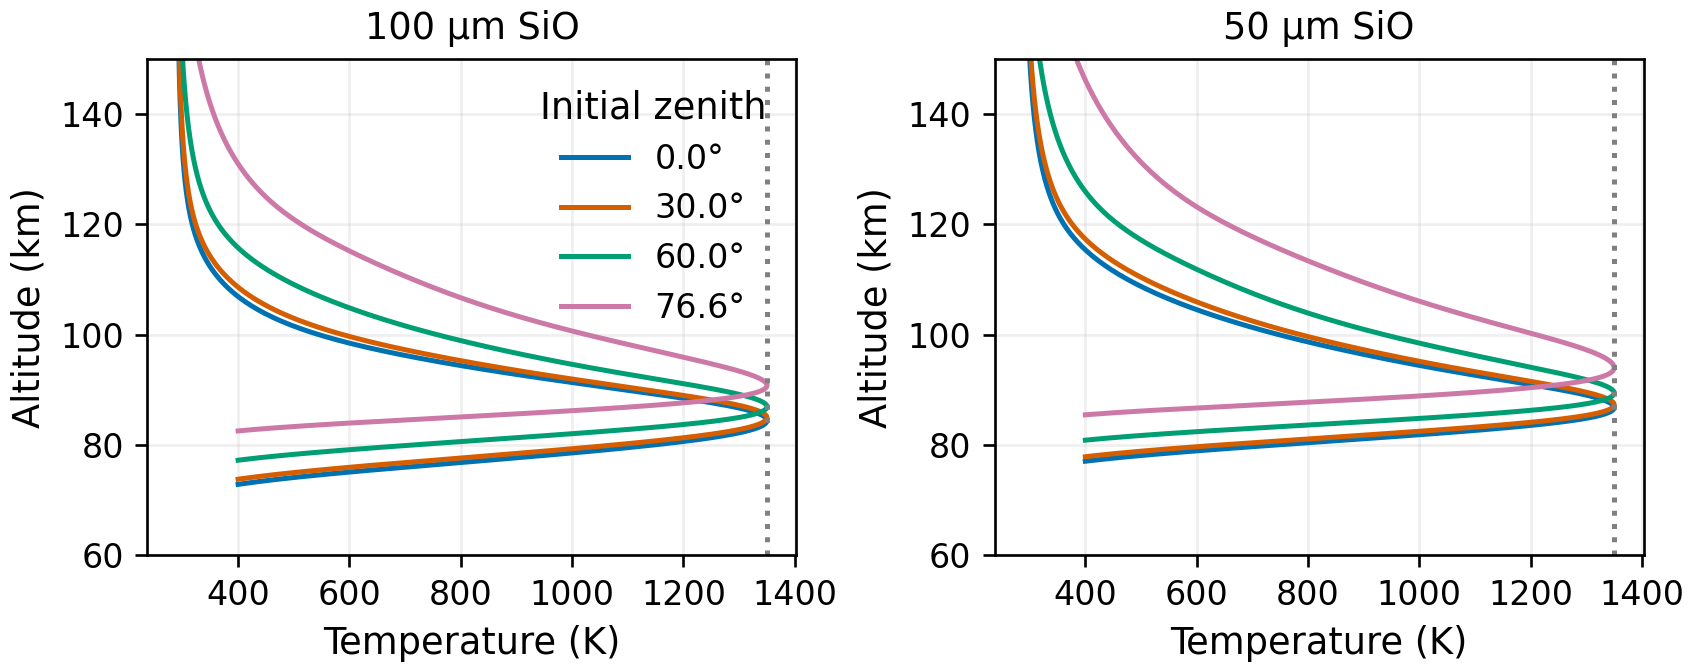
\includegraphics[width=\textwidth]{report_profiles.png}
\caption{Vibe temperature profiles at the 1350 K thresholds. Curves show the
fixed-ray model for four initial zenith angles.}
\scriptprovenance{scripts/report\_metablate.py; data: scripts/run\_metablate.py}
\end{figure}

\newpage
\mmsection{5. Numerical validation: agreement, refinement, and old-output differences}

The 260 numerical assertions comprise 195 kernel/coordinate/atmosphere/event
checks, 63 trajectory/refinement checks (seven per case), and two radiation
array comparisons. An assertion may compare many samples. Additional checks
cover output-capacity failure and atomic rejection of a dimensionally invalid
transaction. The compiler's 22 tests and shell smoke tests pass; a separate
undefined-behavior-sanitized validation run also passes.

Nine trajectories were compared against \emph{the original metablate RHS},
independently integrated with SciPy at matched component tolerances. They cover
50/100 $\mu$m particles, vertical/shallow entries, strong ablation, and the three
largest relevant discrepancies found in saved studies. The comparison uses
SciPy dense output at Vibe sample times within the common interval. Both share
model constants and the input atmosphere, so this tests implementation agreement,
not independent validation of the underlying physics.

\begin{center}
\begin{tabular}{@{}lrl@{}}
\toprule
Quantity & Largest observed difference & Acceptance criterion \\
\midrule
Temperature & 0.004755 K & 0.1 K absolute \\
Mass fraction & $1.3683\times10^{-6}$ & $2\times10^{-5}$ absolute \\
Speed & 0.006809 m/s & $2\times10^{-5}$ relative + 0.02 m/s \\
Signed distance & 0.007791 m & 2 m absolute \\
Terminal time & $6.947\times10^{-6}$ s & 0.002 s absolute \\
Refined peak temperature & 0.07950 K & 0.15 K absolute \\
Refined retained fraction & $4.875\times10^{-7}$ & $2\times10^{-5}$ absolute \\
\bottomrule
\end{tabular}
\end{center}
Refinement reduces relative/absolute tolerances by 100 and maximum step by four.
These are \textbf{empirical error estimates}, not rigorous error bounds, and are
not Vibe's automatic uncertainty-propagation feature. No claim of exhaustive
parameter-space validation is made.

\begin{figure}[H]
\centering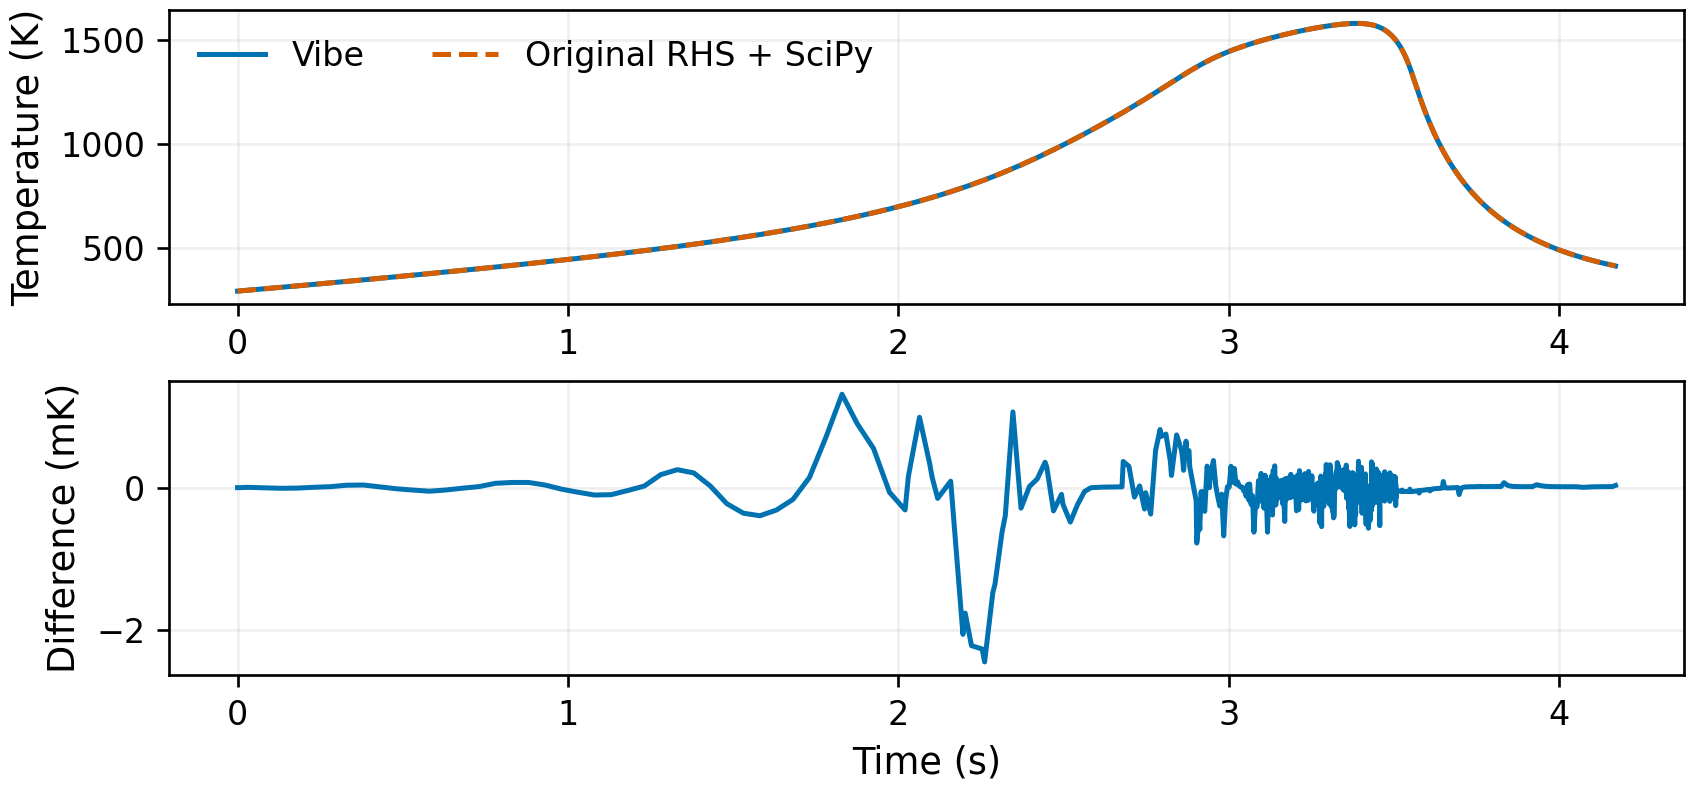
\includegraphics[width=\textwidth]{report_validation.png}
\caption{A challenging historical-discrepancy case: 20 $\mu$m SiO,
25.5 km/s, vertical entry. The tight original-RHS reference and Vibe agree;
their temperature difference is shown in millikelvin below.}
\scriptprovenance{scripts/report\_metablate.py; data: scripts/run\_metablate.py}
\end{figure}

Saved loose-tolerance outputs are not exactly reproduced: the mass/velocity
sweep differs by up to 25.8045 K and 0.0102712 in retained mass fraction;
the emissivity sweep differs by up to 22.4817 K. Tight independent comparisons
pass at those selected worst cases. The legacy solver used scalar absolute
tolerance $10^{-6}$ even for microscopic SI masses, whereas this run resolves
mass fraction. This supports a numerical-tolerance explanation, but is not an
exhaustive attribution of every difference. The local Stefan--Boltzmann
correction is preserved; the old distance-based ground event is corrected to
actual WGS84 altitude. Historical deltas remain in HDF5 for inspection.

\newpage
\mmsection{6. Reproduced scientific studies and interpretation limits}

The run covers non-melt profiles and enhanced-speed comparisons (48 trajectories),
survival boundaries and comparisons (18), the mass/velocity grid (357),
escape-speed angle/size cases (18), and parameter sensitivity (80). The
radiation-pressure/PR calculation adds 1201 native evaluations. Boundary
searches include temperature, retained fraction, and parameter objectives;
two extra cached searches arise from slightly different archived tangent angles.

\begin{figure}[H]
\centering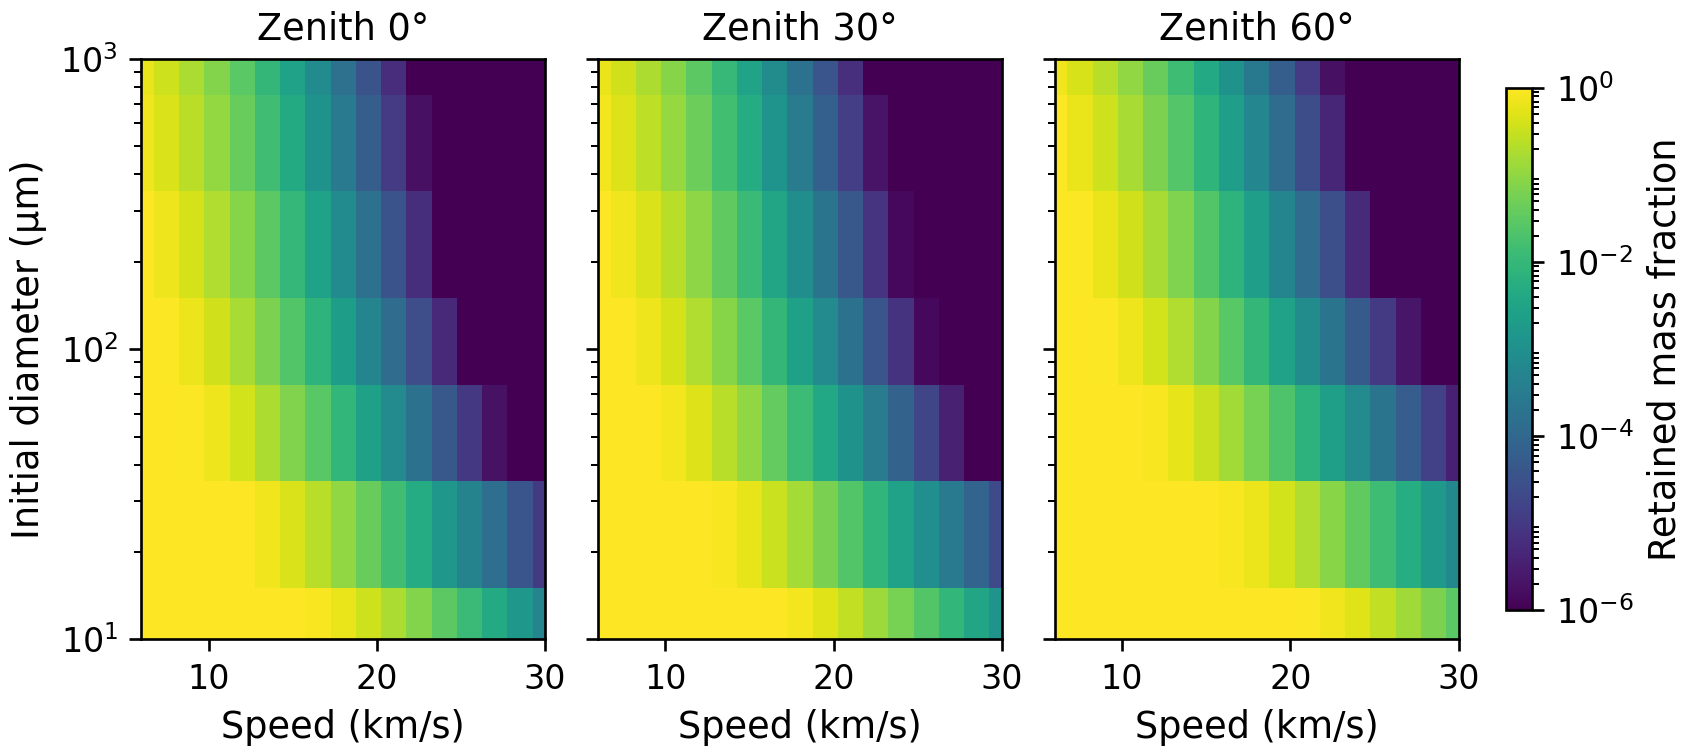
\includegraphics[width=\textwidth]{report_survival.png}
\caption{Retained mass fraction from the 357 Vibe trajectories, displayed on
the sampled diameter/speed grid rather than as a fine-resolution physical
boundary. The display floor is $10^{-6}$; unmodified numerical values are
retained in HDF5.}
\scriptprovenance{scripts/report\_metablate.py; data: scripts/run\_metablate.py}
\end{figure}

\begin{center}
\begin{tabular}{@{}lrrr@{}}
\toprule
100 $\mu$m survival speed (km/s) & 1\% retained & 10\% retained & 50\% retained \\
\midrule
$z=0^\circ$ & 16.125 & 12.871 & 9.737 \\
$z=30^\circ$ & 16.423 & 13.166 & 10.036 \\
$z=60^\circ$ & 17.904 & 14.596 & 11.460 \\
\bottomrule
\end{tabular}
\end{center}
These nine boundaries satisfy the study's 3000 K ceiling. They are thermal
survival criteria in this model, not predictions of mineralogy or melt fraction.
Smaller particles and shallower rays generally tolerate higher initial speed,
but the finite grid is not evidence of behavior between every sampled point.

At the local escape speed, 11.04119 km/s, the vertical 100 $\mu$m sensitivity
searches place the 1350 K crossing at $\Lambda\simeq0.23655$,
$\Gamma\simeq4.05946$, or $\rho_m\simeq537.57\ \mathrm{kg\,m^{-3}}$ when
varied separately. These are diagnostic parameter variations, \emph{not}
adopted material values or a recommendation to increase drag artificially.
The baseline remains $\Lambda=\Gamma=1$.

\mmsection{What this study does not establish}

There is no gravity-curved orbital propagation, capture history, coupled
phase-transition model, material-parameter uncertainty propagation, or empirical
atmospheric validation here. In particular, the tangency column in the threshold
table cannot establish temporary capture or an aerocapture mechanism. Numerical
agreement cannot make a simplified physical model more complete.

The generated study figures also include escape-angle profiles, sensitivity,
and radiation pressure. They are available beside the consolidated HDF5 rather
than all being reduced to unreadable thumbnails in this report. Report plots
are generated at the actual 7.06-inch LaTeX width with 10--11 pt plot text.

\newpage
\mmsection{7. CPU performance and engineering assessment}

On this Apple M4 Pro (arm64, macOS 26.6.2, Apple Clang 21.0.0, Python 3.13.1),
a warmed serial batch of the nine validation cases was timed three times,
alternating implementation order. Compilation, atmosphere construction,
plotting and reference resampling were excluded. Vibe timing includes host
checks, trajectory allocation/copy and native integration; SciPy timing includes
its original Python RHS and dense integration output. Component tolerances and
maximum steps match, but the two adaptive solvers need not take identical steps.

\begin{center}
\begin{tabular}{@{}lrr@{}}
\toprule
Nine-case batch & Median wall time & Observed range \\
\midrule
Compiled Vibe & 8.608 ms & 8.412--8.797 ms \\
Original RHS / SciPy & 4.191 s & 4.161--4.209 s \\
\bottomrule
\end{tabular}
\end{center}
The median ratio is \textbf{487$\times$ for these implementations on this host}.
This primarily demonstrates the value of keeping the repeated numerical work
in compiled code instead of invoking the existing Python/object-heavy RHS.
It is not a comparison with optimized NumPy, Numba, C++, or another native solver,
nor a general language speed ranking. The full study/validation/plot phase took
9.04 s in its recorded run, excluding initial compilation and atmosphere setup;
that mixed workflow time is not a kernel benchmark.

\textbf{What worked.} Typed semantic transactions produced a portable program;
strict scalar types and checked SI interfaces caught invalid calls; explicit
control flow expressed adaptive numerical work; native output reproduced
independent references. A small runtime-checked numerical core was sufficient
for a useful scientific application.

\textbf{What was awkward.} The implementation required compiler extensions and
a custom Python authoring/ABI helper. State and configuration remain positional,
mixed-quantity \texttt{f64} arrays, not named dimension-typed records. The host
checks mutable-buffer overlap, but there is no general ownership proof.
Bounds failures terminate the native process rather than returning structured
agent diagnostics. Peak extraction and tolerances are hand-designed.

\textbf{What is unmeasured.} This task does not measure LLM token consumption,
first-pass validity, repair rate, concurrent-agent throughput, incremental rebuild
cost or large-project scaling. The current pack still undergoes whole-pack
validation/rewriting, and this host regenerates/compiles the whole program.
GPU execution, AD, automatic uncertainty propagation and a production solver
library are not implemented by this port.

\mmsection{8. Recommended next language work}

Prioritize named records with per-field units and generated ABI bindings;
reusable solver/event/result objects with structured failure evidence; semantic
test and convergence records tied to exact revisions; and incremental function
checking/code generation. Then benchmark agent editing/debugging against a
Python baseline. Accelerator work should follow explicit array shapes,
ownership and transfer semantics, not a promise inferred from CPU success.

\mmsection{9. Reproducibility and source record}

From \texttt{/Users/jvi019/src/vibec}, after installing the original study's
dependencies in base conda:
\begin{lstlisting}
cargo build
cargo test
bash scripts/test.sh
conda run -n base python scripts/run_metablate.py
conda run -n base python scripts/report_metablate.py
make -C reports/metablate
\end{lstlisting}

\newpage
\mmsection{10. Artifact map and audit details}

\begin{description}[style=nextline,leftmargin=0pt,labelwidth=0pt,labelsep=0pt]
\item[Executable semantic program]
\path{examples/metablate/metablate.vibepack}: canonical program and semantic
history. It can be checked or inspected with \texttt{vibec env}; no source-text
reconstruction is needed to execute it.
\item[Authoring and native host]
\path{scripts/author_metablate.py}, \path{scripts/semantic_builder.py}, and
\path{scripts/metablate_native.py}. The authoring script embeds RK45 coefficients
from the installed SciPy table as constant semantic expressions. The host pins
the semantic revision before C emission and ABI inspection.
\item[Study runner and input/reference locations]
\path{scripts/run_metablate.py}; original package:
\path{/Users/jvi019/src/ablate}; study definitions and archived references:
\path{/Users/jvi019/src/ablatemm}. The runner records source hashes and the
package commit, including compiler dirty-worktree status rather than claiming
an uncommitted compiler change is already reproducible from a Git commit alone.
\item[Consolidated numerical product]
\path{/Users/jvi019/src/ablatemm/output_vibe/metablate_vibe.h5}. Groups include
atmosphere, nonmelt, survival, escape, sensitivity, radiation, validation and
provenance. The record stores raw trajectories, tolerances, historical differences,
independent reference samples, revision and native build information.
\item[Report and timing evidence]
\path{reports/metablate/report.tex}; figures and
\path{output/pdf/metablate/report_evidence.h5} are created by
\path{scripts/report_metablate.py}. The latter stores all timing repetitions,
host/compiler details, numerical maxima and a hash of the source HDF5.
\end{description}

\mmsection{Pinned program revision for the reported run}
\begin{lstlisting}
sha256:67d5b3c0be9bac23c631605faf2fc8dc6e3334642b9da9aedb5614e652011023
\end{lstlisting}
The exact source and generated-C hashes are retained in HDF5. The report's
rounded tables describe this recorded run; regenerated measurements should be
checked against the report before publishing a new revision.

\mmsection{Additional verification command}
\begin{lstlisting}
conda run -n base python scripts/run_metablate.py 
  --validate-only --sanitize --output target/metablate-sanitize
\end{lstlisting}
Join these two displayed lines for a shell invocation. This enables undefined
behavior checks on the emitted native model. It supplements, rather than
replaces, the numerical comparisons and compiler regression tests.

\mmsection{Source attribution and validation scope}

Physics and coordinates are adapted from the specified metablate checkout,
associated with Daniel Kastinen and Johan Kero, chiefly
\path{models/kero_szasz_2008.py}, \path{physics/thermal_ablation.py} and
\path{coordinates.py}. Study definitions are
\path{model_sio.py}, \path{model_sio_survival.py},
\path{memo001_nonmelt_profiles.py}, \path{model_sio_escape_angle.py},
\path{model_sio_parameter_sensitivity.py} and \path{radiation_pressure_pr.py}.
The derived example includes the upstream GPL license. This report is an
implementation audit of those local sources, not a new literature review or
an independent determination of SiO material properties.

\begin{mmconclusion}
Vibe did well as a compiled numerical substrate once the missing control-flow
and math facilities were added. The strongest evidence is reproducible numerical
agreement and a complete native study loop. The next challenge is making that
result routine for agents: typed records, reusable numerical services, structured
debugging evidence and measured incremental/concurrent development.
\end{mmconclusion}
\end{document}
